\textbf{COLUNI 2026 -- Questão 11}\par\medskip Uma empresa deseja modificar seu slogan, passando de um quadrado para um setor circular. O slogan atual é um quadrado de lado $\ell$ e possui uma listra preta, no formato retangular, em sua parte superior, como indicado na Figura 1. Deseja-se que o novo slogan possua uma região preta no formato de um setor circular de raio $x$, $x<\ell$ e ângulo $30^\circ$, conforme Figura 2.

% COLUNI-AUTO-FIGURES-BEGIN
\begin{figure}[htbp]
\centering
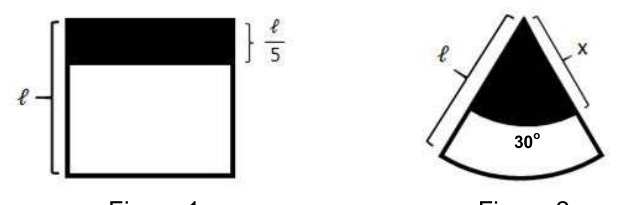
\includegraphics[width=0.75\linewidth]{static/simulados/coluni/figuras/2026/questao-11/figura-1.png}
\end{figure}
% COLUNI-AUTO-FIGURES-END

Considere as medidas $\ell$ e $x$ em centímetros. Para que as regiões indicadas nos slogans na cor preta tenham mesmas áreas, é CORRETO afirmar que o valor de $x$, em centímetros, é:
\begin{enumerate}
\item $\dfrac{\ell\sqrt{15\pi}}{5\pi}$
\item $\dfrac{2\ell\sqrt{15\pi}}{5\pi}$
\item $\dfrac{\ell\sqrt{15}}{5}$
\item $\dfrac{2\ell\sqrt{15}}{5}$
\end{enumerate}
